% Generated by Sphinx.
\def\sphinxdocclass{report}
\documentclass[letterpaper,10pt,english]{sphinxmanual}
\usepackage[utf8]{inputenc}
\DeclareUnicodeCharacter{00A0}{\nobreakspace}
\usepackage{cmap}
\usepackage[T1]{fontenc}
\usepackage{babel}
\usepackage{times}
\usepackage[Bjarne]{fncychap}
\usepackage{longtable}
\usepackage{sphinx}
\usepackage{multirow}


\title{adenine Documentation}
\date{April 04, 2016}
\release{0.1.0}
\author{Samuele Fiorini}
\newcommand{\sphinxlogo}{}
\renewcommand{\releasename}{Release}
\makeindex

\makeatletter
\def\PYG@reset{\let\PYG@it=\relax \let\PYG@bf=\relax%
    \let\PYG@ul=\relax \let\PYG@tc=\relax%
    \let\PYG@bc=\relax \let\PYG@ff=\relax}
\def\PYG@tok#1{\csname PYG@tok@#1\endcsname}
\def\PYG@toks#1+{\ifx\relax#1\empty\else%
    \PYG@tok{#1}\expandafter\PYG@toks\fi}
\def\PYG@do#1{\PYG@bc{\PYG@tc{\PYG@ul{%
    \PYG@it{\PYG@bf{\PYG@ff{#1}}}}}}}
\def\PYG#1#2{\PYG@reset\PYG@toks#1+\relax+\PYG@do{#2}}

\expandafter\def\csname PYG@tok@gd\endcsname{\def\PYG@tc##1{\textcolor[rgb]{0.63,0.00,0.00}{##1}}}
\expandafter\def\csname PYG@tok@gu\endcsname{\let\PYG@bf=\textbf\def\PYG@tc##1{\textcolor[rgb]{0.50,0.00,0.50}{##1}}}
\expandafter\def\csname PYG@tok@gt\endcsname{\def\PYG@tc##1{\textcolor[rgb]{0.00,0.27,0.87}{##1}}}
\expandafter\def\csname PYG@tok@gs\endcsname{\let\PYG@bf=\textbf}
\expandafter\def\csname PYG@tok@gr\endcsname{\def\PYG@tc##1{\textcolor[rgb]{1.00,0.00,0.00}{##1}}}
\expandafter\def\csname PYG@tok@cm\endcsname{\let\PYG@it=\textit\def\PYG@tc##1{\textcolor[rgb]{0.25,0.50,0.56}{##1}}}
\expandafter\def\csname PYG@tok@vg\endcsname{\def\PYG@tc##1{\textcolor[rgb]{0.73,0.38,0.84}{##1}}}
\expandafter\def\csname PYG@tok@m\endcsname{\def\PYG@tc##1{\textcolor[rgb]{0.13,0.50,0.31}{##1}}}
\expandafter\def\csname PYG@tok@mh\endcsname{\def\PYG@tc##1{\textcolor[rgb]{0.13,0.50,0.31}{##1}}}
\expandafter\def\csname PYG@tok@cs\endcsname{\def\PYG@tc##1{\textcolor[rgb]{0.25,0.50,0.56}{##1}}\def\PYG@bc##1{\setlength{\fboxsep}{0pt}\colorbox[rgb]{1.00,0.94,0.94}{\strut ##1}}}
\expandafter\def\csname PYG@tok@ge\endcsname{\let\PYG@it=\textit}
\expandafter\def\csname PYG@tok@vc\endcsname{\def\PYG@tc##1{\textcolor[rgb]{0.73,0.38,0.84}{##1}}}
\expandafter\def\csname PYG@tok@il\endcsname{\def\PYG@tc##1{\textcolor[rgb]{0.13,0.50,0.31}{##1}}}
\expandafter\def\csname PYG@tok@go\endcsname{\def\PYG@tc##1{\textcolor[rgb]{0.20,0.20,0.20}{##1}}}
\expandafter\def\csname PYG@tok@cp\endcsname{\def\PYG@tc##1{\textcolor[rgb]{0.00,0.44,0.13}{##1}}}
\expandafter\def\csname PYG@tok@gi\endcsname{\def\PYG@tc##1{\textcolor[rgb]{0.00,0.63,0.00}{##1}}}
\expandafter\def\csname PYG@tok@gh\endcsname{\let\PYG@bf=\textbf\def\PYG@tc##1{\textcolor[rgb]{0.00,0.00,0.50}{##1}}}
\expandafter\def\csname PYG@tok@ni\endcsname{\let\PYG@bf=\textbf\def\PYG@tc##1{\textcolor[rgb]{0.84,0.33,0.22}{##1}}}
\expandafter\def\csname PYG@tok@nl\endcsname{\let\PYG@bf=\textbf\def\PYG@tc##1{\textcolor[rgb]{0.00,0.13,0.44}{##1}}}
\expandafter\def\csname PYG@tok@nn\endcsname{\let\PYG@bf=\textbf\def\PYG@tc##1{\textcolor[rgb]{0.05,0.52,0.71}{##1}}}
\expandafter\def\csname PYG@tok@no\endcsname{\def\PYG@tc##1{\textcolor[rgb]{0.38,0.68,0.84}{##1}}}
\expandafter\def\csname PYG@tok@na\endcsname{\def\PYG@tc##1{\textcolor[rgb]{0.25,0.44,0.63}{##1}}}
\expandafter\def\csname PYG@tok@nb\endcsname{\def\PYG@tc##1{\textcolor[rgb]{0.00,0.44,0.13}{##1}}}
\expandafter\def\csname PYG@tok@nc\endcsname{\let\PYG@bf=\textbf\def\PYG@tc##1{\textcolor[rgb]{0.05,0.52,0.71}{##1}}}
\expandafter\def\csname PYG@tok@nd\endcsname{\let\PYG@bf=\textbf\def\PYG@tc##1{\textcolor[rgb]{0.33,0.33,0.33}{##1}}}
\expandafter\def\csname PYG@tok@ne\endcsname{\def\PYG@tc##1{\textcolor[rgb]{0.00,0.44,0.13}{##1}}}
\expandafter\def\csname PYG@tok@nf\endcsname{\def\PYG@tc##1{\textcolor[rgb]{0.02,0.16,0.49}{##1}}}
\expandafter\def\csname PYG@tok@si\endcsname{\let\PYG@it=\textit\def\PYG@tc##1{\textcolor[rgb]{0.44,0.63,0.82}{##1}}}
\expandafter\def\csname PYG@tok@s2\endcsname{\def\PYG@tc##1{\textcolor[rgb]{0.25,0.44,0.63}{##1}}}
\expandafter\def\csname PYG@tok@vi\endcsname{\def\PYG@tc##1{\textcolor[rgb]{0.73,0.38,0.84}{##1}}}
\expandafter\def\csname PYG@tok@nt\endcsname{\let\PYG@bf=\textbf\def\PYG@tc##1{\textcolor[rgb]{0.02,0.16,0.45}{##1}}}
\expandafter\def\csname PYG@tok@nv\endcsname{\def\PYG@tc##1{\textcolor[rgb]{0.73,0.38,0.84}{##1}}}
\expandafter\def\csname PYG@tok@s1\endcsname{\def\PYG@tc##1{\textcolor[rgb]{0.25,0.44,0.63}{##1}}}
\expandafter\def\csname PYG@tok@gp\endcsname{\let\PYG@bf=\textbf\def\PYG@tc##1{\textcolor[rgb]{0.78,0.36,0.04}{##1}}}
\expandafter\def\csname PYG@tok@sh\endcsname{\def\PYG@tc##1{\textcolor[rgb]{0.25,0.44,0.63}{##1}}}
\expandafter\def\csname PYG@tok@ow\endcsname{\let\PYG@bf=\textbf\def\PYG@tc##1{\textcolor[rgb]{0.00,0.44,0.13}{##1}}}
\expandafter\def\csname PYG@tok@sx\endcsname{\def\PYG@tc##1{\textcolor[rgb]{0.78,0.36,0.04}{##1}}}
\expandafter\def\csname PYG@tok@bp\endcsname{\def\PYG@tc##1{\textcolor[rgb]{0.00,0.44,0.13}{##1}}}
\expandafter\def\csname PYG@tok@c1\endcsname{\let\PYG@it=\textit\def\PYG@tc##1{\textcolor[rgb]{0.25,0.50,0.56}{##1}}}
\expandafter\def\csname PYG@tok@kc\endcsname{\let\PYG@bf=\textbf\def\PYG@tc##1{\textcolor[rgb]{0.00,0.44,0.13}{##1}}}
\expandafter\def\csname PYG@tok@c\endcsname{\let\PYG@it=\textit\def\PYG@tc##1{\textcolor[rgb]{0.25,0.50,0.56}{##1}}}
\expandafter\def\csname PYG@tok@mf\endcsname{\def\PYG@tc##1{\textcolor[rgb]{0.13,0.50,0.31}{##1}}}
\expandafter\def\csname PYG@tok@err\endcsname{\def\PYG@bc##1{\setlength{\fboxsep}{0pt}\fcolorbox[rgb]{1.00,0.00,0.00}{1,1,1}{\strut ##1}}}
\expandafter\def\csname PYG@tok@kd\endcsname{\let\PYG@bf=\textbf\def\PYG@tc##1{\textcolor[rgb]{0.00,0.44,0.13}{##1}}}
\expandafter\def\csname PYG@tok@ss\endcsname{\def\PYG@tc##1{\textcolor[rgb]{0.32,0.47,0.09}{##1}}}
\expandafter\def\csname PYG@tok@sr\endcsname{\def\PYG@tc##1{\textcolor[rgb]{0.14,0.33,0.53}{##1}}}
\expandafter\def\csname PYG@tok@mo\endcsname{\def\PYG@tc##1{\textcolor[rgb]{0.13,0.50,0.31}{##1}}}
\expandafter\def\csname PYG@tok@mi\endcsname{\def\PYG@tc##1{\textcolor[rgb]{0.13,0.50,0.31}{##1}}}
\expandafter\def\csname PYG@tok@kn\endcsname{\let\PYG@bf=\textbf\def\PYG@tc##1{\textcolor[rgb]{0.00,0.44,0.13}{##1}}}
\expandafter\def\csname PYG@tok@o\endcsname{\def\PYG@tc##1{\textcolor[rgb]{0.40,0.40,0.40}{##1}}}
\expandafter\def\csname PYG@tok@kr\endcsname{\let\PYG@bf=\textbf\def\PYG@tc##1{\textcolor[rgb]{0.00,0.44,0.13}{##1}}}
\expandafter\def\csname PYG@tok@s\endcsname{\def\PYG@tc##1{\textcolor[rgb]{0.25,0.44,0.63}{##1}}}
\expandafter\def\csname PYG@tok@kp\endcsname{\def\PYG@tc##1{\textcolor[rgb]{0.00,0.44,0.13}{##1}}}
\expandafter\def\csname PYG@tok@w\endcsname{\def\PYG@tc##1{\textcolor[rgb]{0.73,0.73,0.73}{##1}}}
\expandafter\def\csname PYG@tok@kt\endcsname{\def\PYG@tc##1{\textcolor[rgb]{0.56,0.13,0.00}{##1}}}
\expandafter\def\csname PYG@tok@sc\endcsname{\def\PYG@tc##1{\textcolor[rgb]{0.25,0.44,0.63}{##1}}}
\expandafter\def\csname PYG@tok@sb\endcsname{\def\PYG@tc##1{\textcolor[rgb]{0.25,0.44,0.63}{##1}}}
\expandafter\def\csname PYG@tok@k\endcsname{\let\PYG@bf=\textbf\def\PYG@tc##1{\textcolor[rgb]{0.00,0.44,0.13}{##1}}}
\expandafter\def\csname PYG@tok@se\endcsname{\let\PYG@bf=\textbf\def\PYG@tc##1{\textcolor[rgb]{0.25,0.44,0.63}{##1}}}
\expandafter\def\csname PYG@tok@sd\endcsname{\let\PYG@it=\textit\def\PYG@tc##1{\textcolor[rgb]{0.25,0.44,0.63}{##1}}}

\def\PYGZbs{\char`\\}
\def\PYGZus{\char`\_}
\def\PYGZob{\char`\{}
\def\PYGZcb{\char`\}}
\def\PYGZca{\char`\^}
\def\PYGZam{\char`\&}
\def\PYGZlt{\char`\<}
\def\PYGZgt{\char`\>}
\def\PYGZsh{\char`\#}
\def\PYGZpc{\char`\%}
\def\PYGZdl{\char`\$}
\def\PYGZhy{\char`\-}
\def\PYGZsq{\char`\'}
\def\PYGZdq{\char`\"}
\def\PYGZti{\char`\~}
% for compatibility with earlier versions
\def\PYGZat{@}
\def\PYGZlb{[}
\def\PYGZrb{]}
\makeatother

\begin{document}

\maketitle
\tableofcontents
\phantomsection\label{index::doc}


\textbf{adenine} is a machine learning and data mining Python pipeline that helps you to answer this tedious question: are my data relevant with the problem I'm dealing with?

The main structure of adenine can be summarized in the following 3 steps.
\begin{enumerate}
\item {} 
\textbf{Preprocessing:} Have you ever wondered what would have changed if only  your data have been preprocessed in a different way? Or is data preprocessing is a good idea at all? adenine offers several preprocessing procedures, such as: data centering, Min-Max scaling, standardization or normalization and allows you to compare the results of the analysis conducted with different starting point.

\item {} 
\textbf{Dimensionality Reduction:} In the context of data exploration, this  phase becomes particularly helpful for high dimensional data (e.g. -omics scenario). This step, generically named DR, may actually include some manifold learning   (such as Isomap, Multidimensional Scaling, etc), supervised (Linear   Discriminant Analysis) and unsupervised (Principal Component Analysis, kernel PCA) techniques.

\item {} 
\textbf{Clustering:} This section aims at grouping data into clusters without taking into account the class labels. Several techniques such as K-Means, Spectral or Hierarchical clustering will work on both original and dimensionality reduced data.

\end{enumerate}

The final output of adenine is a compact and textual representation of the results obtained from the pipelines made with each possible combination of the algorithms
implemented at each step.


\chapter{User documentation}
\label{index:adenine-a-data-exploration-pipeline}\label{index:user-documentation}

\section{Quick start tutorial}
\label{tutorial::doc}\label{tutorial:quick-start-tutorial}\label{tutorial:tutorial}
\textbf{adenine} may be installed using standard Python tools (with
administrative or sudo permissions on GNU-Linux platforms):

\begin{Verbatim}[commandchars=\\\{\}]
\PYGZdl{} pip install adenine

or

\PYGZdl{} easy\PYGZus{}install adenine
\end{Verbatim}


\subsection{Installation from sources}
\label{tutorial:installation-from-sources}
If you like to manually install \textbf{adenine}, download the source tar.gz
from our
\href{https://bitbucket.org/samuele\_fiorini/adenine}{BitBucket repository}.
Then extract it and move into the root directory:

\begin{Verbatim}[commandchars=\\\{\}]
\PYGZdl{} tar xvf adenine\PYGZhy{}\textbar{}release\textbar{}.tar.gz
\PYGZdl{} cd adenine\PYGZhy{}\textbar{}release\textbar{}/
\end{Verbatim}

From here, you may use the standard Python installation step:

\begin{Verbatim}[commandchars=\\\{\}]
\PYGZdl{} python setup.py install
\end{Verbatim}

After \textbf{adenine} installation, you should have access to two scripts,
named with a common \code{ade\_} prefix:

\begin{Verbatim}[commandchars=\\\{\}]
\PYGZdl{} ade\PYGZus{}\PYGZlt{}TAB\PYGZgt{}
ade\PYGZus{}analysis.py    ade\PYGZus{}run.py
\end{Verbatim}

This tutorial assumes that you downloaded and extracted \textbf{adenine}
source package which contains a \code{examples} directory with some \code{.npy} files
which will be used to show \textbf{adenine}`s' functionalities.

\textbf{adenine} needs only 3 ingredients:
\begin{itemize}
\item {} 
A \code{X.npy} input matrix

\item {} 
A \code{y.npy} output vector (optional)

\item {} 
A \code{configuration} file

\end{itemize}


\subsection{Input data format}
\label{tutorial:input-data-format}
Input data are assumed to be \code{numpy} array dumped in a \code{.npy} files organized with a row for each sample and a column for each feature.


\subsection{Configuration File}
\label{tutorial:configuration-file}\label{tutorial:configuration}
\textbf{adenine} configuration file is a standard Python script. It is
imported as a module, then all the code is executed. In this file the user can define all the option needed to read the data and to create the pipelines.

\begin{Verbatim}[commandchars=\\\{\}]
\PYG{c}{\PYGZsh{}!/usr/bin/python}
\PYG{c}{\PYGZsh{} \PYGZhy{}*\PYGZhy{} coding: utf\PYGZhy{}8 \PYGZhy{}*\PYGZhy{}}

\PYG{k+kn}{from} \PYG{n+nn}{adenine.utils} \PYG{k+kn}{import} \PYG{n}{data\PYGZus{}source}

\PYG{c}{\PYGZsh{} \PYGZhy{}\PYGZhy{}\PYGZhy{}\PYGZhy{}\PYGZhy{}\PYGZhy{}\PYGZhy{}\PYGZhy{}\PYGZhy{}\PYGZhy{}\PYGZhy{}\PYGZhy{}\PYGZhy{}\PYGZhy{}\PYGZhy{}\PYGZhy{}\PYGZhy{}\PYGZhy{}\PYGZhy{}\PYGZhy{}\PYGZhy{}\PYGZhy{}\PYGZhy{}\PYGZhy{}\PYGZhy{}\PYGZhy{}  EXPERMIENT INFO \PYGZhy{}\PYGZhy{}\PYGZhy{}\PYGZhy{}\PYGZhy{}\PYGZhy{}\PYGZhy{}\PYGZhy{}\PYGZhy{}\PYGZhy{}\PYGZhy{}\PYGZhy{}\PYGZhy{}\PYGZhy{}\PYGZhy{}\PYGZhy{}\PYGZhy{}\PYGZhy{}\PYGZhy{}\PYGZhy{}\PYGZhy{}\PYGZhy{}\PYGZhy{}\PYGZhy{}\PYGZhy{} \PYGZsh{}}
\PYG{n}{exp\PYGZus{}tag} \PYG{o}{=} \PYG{l+s}{\PYGZsq{}}\PYG{l+s}{debug\PYGZus{}csv}\PYG{l+s}{\PYGZsq{}}
\PYG{n}{output\PYGZus{}root\PYGZus{}folder} \PYG{o}{=} \PYG{l+s}{\PYGZsq{}}\PYG{l+s}{results}\PYG{l+s}{\PYGZsq{}}
\PYG{c}{\PYGZsh{} parallel = False}

\PYG{c}{\PYGZsh{} \PYGZhy{}\PYGZhy{}\PYGZhy{}\PYGZhy{}\PYGZhy{}\PYGZhy{}\PYGZhy{}\PYGZhy{}\PYGZhy{}\PYGZhy{}\PYGZhy{}\PYGZhy{}\PYGZhy{}\PYGZhy{}\PYGZhy{}\PYGZhy{}\PYGZhy{}\PYGZhy{}\PYGZhy{}\PYGZhy{}\PYGZhy{}\PYGZhy{}\PYGZhy{}\PYGZhy{}\PYGZhy{}\PYGZhy{}\PYGZhy{}\PYGZhy{}  INPUT DATA \PYGZhy{}\PYGZhy{}\PYGZhy{}\PYGZhy{}\PYGZhy{}\PYGZhy{}\PYGZhy{}\PYGZhy{}\PYGZhy{}\PYGZhy{}\PYGZhy{}\PYGZhy{}\PYGZhy{}\PYGZhy{}\PYGZhy{}\PYGZhy{}\PYGZhy{}\PYGZhy{}\PYGZhy{}\PYGZhy{}\PYGZhy{}\PYGZhy{}\PYGZhy{}\PYGZhy{}\PYGZhy{}\PYGZhy{}\PYGZhy{}\PYGZhy{} \PYGZsh{}}
\PYG{c}{\PYGZsh{} X, y, feat\PYGZus{}names, class\PYGZus{}names = data\PYGZus{}source.load(\PYGZsq{}iris\PYGZsq{})}
\PYG{c}{\PYGZsh{} X, y, feat\PYGZus{}names, class\PYGZus{}names = data\PYGZus{}source.load(\PYGZsq{}gauss\PYGZsq{})}
\PYG{c}{\PYGZsh{} X, y, feat\PYGZus{}names, class\PYGZus{}names = data\PYGZus{}source.load(\PYGZsq{}digits\PYGZsq{})}
\PYG{c}{\PYGZsh{} X, y, feat\PYGZus{}names, class\PYGZus{}names = data\PYGZus{}source.load(\PYGZsq{}diabetes\PYGZsq{})}
\PYG{c}{\PYGZsh{} X, y, feat\PYGZus{}names, class\PYGZus{}names = data\PYGZus{}source.load(\PYGZsq{}boston\PYGZsq{})}
\PYG{c}{\PYGZsh{} X, y, feat\PYGZus{}names, class\PYGZus{}names = data\PYGZus{}source.load(\PYGZsq{}custom\PYGZsq{}, \PYGZsq{}X.npy\PYGZsq{}, \PYGZsq{}y.npy\PYGZsq{})}
\PYG{c}{\PYGZsh{} X, y, feat\PYGZus{}names, class\PYGZus{}names = data\PYGZus{}source.load(\PYGZsq{}custom\PYGZsq{}, \PYGZsq{}X.csv\PYGZsq{}, \PYGZsq{}y.csv\PYGZsq{})}
\PYG{n}{X}\PYG{p}{,} \PYG{n}{y}\PYG{p}{,} \PYG{n}{feat\PYGZus{}names}\PYG{p}{,} \PYG{n}{class\PYGZus{}names} \PYG{o}{=} \PYG{n}{data\PYGZus{}source}\PYG{o}{.}\PYG{n}{load}\PYG{p}{(}\PYG{l+s}{\PYGZsq{}}\PYG{l+s}{custom}\PYG{l+s}{\PYGZsq{}}\PYG{p}{,} \PYG{l+s}{\PYGZsq{}}\PYG{l+s}{/home/fede/src/adenine/adenine/examples/TM\PYGZus{}matrix.csv}\PYG{l+s}{\PYGZsq{}}\PYG{p}{)}
\PYG{k}{if} \PYG{o+ow}{not} \PYG{p}{(}\PYG{n}{X}\PYG{o}{.}\PYG{n}{T} \PYG{o}{==} \PYG{n}{X}\PYG{p}{)}\PYG{o}{.}\PYG{n}{all}\PYG{p}{(}\PYG{p}{)}\PYG{p}{:}
    \PYG{n}{X} \PYG{o}{=} \PYG{p}{(}\PYG{n}{X}\PYG{o}{.}\PYG{n}{T} \PYG{o}{+} \PYG{n}{X}\PYG{p}{)} \PYG{o}{/} \PYG{l+m+mf}{2.}
    \PYG{n}{X} \PYG{o}{=} \PYG{l+m+mf}{1.} \PYG{o}{\PYGZhy{}} \PYG{n}{X}

\PYG{c}{\PYGZsh{} \PYGZhy{}\PYGZhy{}\PYGZhy{}\PYGZhy{}\PYGZhy{}\PYGZhy{}\PYGZhy{}\PYGZhy{}\PYGZhy{}\PYGZhy{}\PYGZhy{}\PYGZhy{}\PYGZhy{}\PYGZhy{}\PYGZhy{}\PYGZhy{}\PYGZhy{}\PYGZhy{}\PYGZhy{}\PYGZhy{}\PYGZhy{}\PYGZhy{}\PYGZhy{}  PIPELINE DEFINITION \PYGZhy{}\PYGZhy{}\PYGZhy{}\PYGZhy{}\PYGZhy{}\PYGZhy{}\PYGZhy{}\PYGZhy{}\PYGZhy{}\PYGZhy{}\PYGZhy{}\PYGZhy{}\PYGZhy{}\PYGZhy{}\PYGZhy{}\PYGZhy{}\PYGZhy{}\PYGZhy{}\PYGZhy{}\PYGZhy{}\PYGZhy{}\PYGZhy{}\PYGZhy{}\PYGZhy{} \PYGZsh{}}

\PYG{c}{\PYGZsh{} \PYGZhy{}\PYGZhy{}\PYGZhy{} Missing Values Imputing \PYGZhy{}\PYGZhy{}\PYGZhy{} \PYGZsh{}}
\PYG{n}{step0} \PYG{o}{=} \PYG{p}{\PYGZob{}}\PYG{l+s}{\PYGZsq{}}\PYG{l+s}{Impute}\PYG{l+s}{\PYGZsq{}}\PYG{p}{:} \PYG{p}{[}\PYG{n+nb+bp}{False}\PYG{p}{]}\PYG{p}{,} \PYG{l+s}{\PYGZsq{}}\PYG{l+s}{Missing}\PYG{l+s}{\PYGZsq{}}\PYG{p}{:} \PYG{p}{[}\PYG{o}{\PYGZhy{}}\PYG{l+m+mi}{1}\PYG{p}{]}\PYG{p}{,} \PYG{l+s}{\PYGZsq{}}\PYG{l+s}{Replacement}\PYG{l+s}{\PYGZsq{}}\PYG{p}{:} \PYG{p}{[}\PYG{l+s}{\PYGZsq{}}\PYG{l+s}{median}\PYG{l+s}{\PYGZsq{}}\PYG{p}{,}\PYG{l+s}{\PYGZsq{}}\PYG{l+s}{mean}\PYG{l+s}{\PYGZsq{}}\PYG{p}{]}\PYG{p}{\PYGZcb{}}

\PYG{c}{\PYGZsh{} \PYGZhy{}\PYGZhy{}\PYGZhy{} Data Preprocessing \PYGZhy{}\PYGZhy{}\PYGZhy{} \PYGZsh{}}
\PYG{n}{step1} \PYG{o}{=} \PYG{p}{\PYGZob{}}\PYG{l+s}{\PYGZsq{}}\PYG{l+s}{None}\PYG{l+s}{\PYGZsq{}}\PYG{p}{:} \PYG{p}{[}\PYG{n+nb+bp}{True}\PYG{p}{]}\PYG{p}{,} \PYG{l+s}{\PYGZsq{}}\PYG{l+s}{Recenter}\PYG{l+s}{\PYGZsq{}}\PYG{p}{:} \PYG{p}{[}\PYG{n+nb+bp}{False}\PYG{p}{]}\PYG{p}{,} \PYG{l+s}{\PYGZsq{}}\PYG{l+s}{Standardize}\PYG{l+s}{\PYGZsq{}}\PYG{p}{:} \PYG{p}{[}\PYG{n+nb+bp}{False}\PYG{p}{]}\PYG{p}{,}
         \PYG{l+s}{\PYGZsq{}}\PYG{l+s}{Normalize}\PYG{l+s}{\PYGZsq{}}\PYG{p}{:} \PYG{p}{[}\PYG{n+nb+bp}{False}\PYG{p}{,} \PYG{p}{[}\PYG{l+s}{\PYGZsq{}}\PYG{l+s}{l2}\PYG{l+s}{\PYGZsq{}}\PYG{p}{]}\PYG{p}{]}\PYG{p}{,} \PYG{l+s}{\PYGZsq{}}\PYG{l+s}{MinMax}\PYG{l+s}{\PYGZsq{}}\PYG{p}{:} \PYG{p}{[}\PYG{n+nb+bp}{False}\PYG{p}{,} \PYG{p}{[}\PYG{l+m+mi}{0}\PYG{p}{,}\PYG{l+m+mi}{1}\PYG{p}{]}\PYG{p}{]}\PYG{p}{\PYGZcb{}}

\PYG{c}{\PYGZsh{} \PYGZhy{}\PYGZhy{}\PYGZhy{} Dimensionality Reduction \PYGZam{} Manifold Learning \PYGZhy{}\PYGZhy{}\PYGZhy{} \PYGZsh{}}
\PYG{n}{step2} \PYG{o}{=} \PYG{p}{\PYGZob{}}\PYG{l+s}{\PYGZsq{}}\PYG{l+s}{PCA}\PYG{l+s}{\PYGZsq{}}\PYG{p}{:} \PYG{p}{[}\PYG{n+nb+bp}{False}\PYG{p}{]}\PYG{p}{,} \PYG{l+s}{\PYGZsq{}}\PYG{l+s}{IncrementalPCA}\PYG{l+s}{\PYGZsq{}}\PYG{p}{:} \PYG{p}{[}\PYG{n+nb+bp}{False}\PYG{p}{]}\PYG{p}{,} \PYG{l+s}{\PYGZsq{}}\PYG{l+s}{RandomizedPCA}\PYG{l+s}{\PYGZsq{}}\PYG{p}{:} \PYG{p}{[}\PYG{n+nb+bp}{False}\PYG{p}{]}\PYG{p}{,}
         \PYG{l+s}{\PYGZsq{}}\PYG{l+s}{KernelPCA}\PYG{l+s}{\PYGZsq{}}\PYG{p}{:} \PYG{p}{[}\PYG{n+nb+bp}{False}\PYG{p}{,} \PYG{p}{[}\PYG{l+s}{\PYGZsq{}}\PYG{l+s}{linear}\PYG{l+s}{\PYGZsq{}}\PYG{p}{,}\PYG{l+s}{\PYGZsq{}}\PYG{l+s}{rbf}\PYG{l+s}{\PYGZsq{}}\PYG{p}{,}\PYG{l+s}{\PYGZsq{}}\PYG{l+s}{poly}\PYG{l+s}{\PYGZsq{}}\PYG{p}{]}\PYG{p}{]}\PYG{p}{,} \PYG{l+s}{\PYGZsq{}}\PYG{l+s}{Isomap}\PYG{l+s}{\PYGZsq{}}\PYG{p}{:} \PYG{p}{[}\PYG{n+nb+bp}{False}\PYG{p}{]}\PYG{p}{,}
         \PYG{l+s}{\PYGZsq{}}\PYG{l+s}{LLE}\PYG{l+s}{\PYGZsq{}}\PYG{p}{:} \PYG{p}{[}\PYG{n+nb+bp}{False}\PYG{p}{,} \PYG{p}{[}\PYG{l+s}{\PYGZsq{}}\PYG{l+s}{standard}\PYG{l+s}{\PYGZsq{}}\PYG{p}{,}\PYG{l+s}{\PYGZsq{}}\PYG{l+s}{modified}\PYG{l+s}{\PYGZsq{}}\PYG{p}{,}\PYG{l+s}{\PYGZsq{}}\PYG{l+s}{hessian}\PYG{l+s}{\PYGZsq{}}\PYG{p}{,} \PYG{l+s}{\PYGZsq{}}\PYG{l+s}{ltsa}\PYG{l+s}{\PYGZsq{}}\PYG{p}{]}\PYG{p}{]}\PYG{p}{,}
         \PYG{l+s}{\PYGZsq{}}\PYG{l+s}{SE}\PYG{l+s}{\PYGZsq{}}\PYG{p}{:} \PYG{p}{[}\PYG{n+nb+bp}{False}\PYG{p}{]}\PYG{p}{,} \PYG{l+s}{\PYGZsq{}}\PYG{l+s}{MDS}\PYG{l+s}{\PYGZsq{}}\PYG{p}{:} \PYG{p}{[}\PYG{n+nb+bp}{False}\PYG{p}{,} \PYG{p}{[}\PYG{l+s}{\PYGZsq{}}\PYG{l+s}{metric}\PYG{l+s}{\PYGZsq{}}\PYG{p}{,}\PYG{l+s}{\PYGZsq{}}\PYG{l+s}{nonmetric}\PYG{l+s}{\PYGZsq{}}\PYG{p}{]}\PYG{p}{]}\PYG{p}{,}
         \PYG{l+s}{\PYGZsq{}}\PYG{l+s}{tSNE}\PYG{l+s}{\PYGZsq{}}\PYG{p}{:} \PYG{p}{[}\PYG{n+nb+bp}{False}\PYG{p}{]}\PYG{p}{,} \PYG{l+s}{\PYGZsq{}}\PYG{l+s}{None}\PYG{l+s}{\PYGZsq{}}\PYG{p}{:} \PYG{p}{[}\PYG{n+nb+bp}{True}\PYG{p}{]}\PYG{p}{\PYGZcb{}}

\PYG{c}{\PYGZsh{} \PYGZhy{}\PYGZhy{}\PYGZhy{} Clustering \PYGZhy{}\PYGZhy{}\PYGZhy{} \PYGZsh{}}
\PYG{n}{step3} \PYG{o}{=} \PYG{p}{\PYGZob{}}\PYG{l+s}{\PYGZsq{}}\PYG{l+s}{KMeans}\PYG{l+s}{\PYGZsq{}}\PYG{p}{:} \PYG{p}{[}\PYG{n+nb+bp}{False}\PYG{p}{,} \PYG{p}{[}\PYG{l+m+mi}{5}\PYG{p}{]}\PYG{p}{]}\PYG{p}{,}
         \PYG{l+s}{\PYGZsq{}}\PYG{l+s}{KernelKMeans}\PYG{l+s}{\PYGZsq{}}\PYG{p}{:} \PYG{p}{[}\PYG{n+nb+bp}{False}\PYG{p}{,} \PYG{p}{[}\PYG{l+m+mi}{3}\PYG{p}{,}\PYG{p}{[}\PYG{l+s}{\PYGZsq{}}\PYG{l+s}{rbf}\PYG{l+s}{\PYGZsq{}}\PYG{p}{,}\PYG{l+s}{\PYGZsq{}}\PYG{l+s}{poly}\PYG{l+s}{\PYGZsq{}}\PYG{p}{]}\PYG{p}{]}\PYG{p}{]}\PYG{p}{,} \PYG{c}{\PYGZsh{}TODO}
         \PYG{l+s}{\PYGZsq{}}\PYG{l+s}{AP}\PYG{l+s}{\PYGZsq{}}\PYG{p}{:} \PYG{p}{[}\PYG{n+nb+bp}{False}\PYG{p}{,} \PYG{p}{[}\PYG{l+s}{\PYGZsq{}}\PYG{l+s}{precomputed}\PYG{l+s}{\PYGZsq{}}\PYG{p}{]}\PYG{p}{]}\PYG{p}{,} \PYG{l+s}{\PYGZsq{}}\PYG{l+s}{MS}\PYG{l+s}{\PYGZsq{}}\PYG{p}{:} \PYG{p}{[}\PYG{n+nb+bp}{False}\PYG{p}{]}\PYG{p}{,}
         \PYG{l+s}{\PYGZsq{}}\PYG{l+s}{Spectral}\PYG{l+s}{\PYGZsq{}}\PYG{p}{:} \PYG{p}{[}\PYG{n+nb+bp}{True}\PYG{p}{,} \PYG{p}{[}\PYG{l+m+mi}{50}\PYG{p}{,} \PYG{p}{[}\PYG{l+s}{\PYGZsq{}}\PYG{l+s}{precomputed}\PYG{l+s}{\PYGZsq{}}\PYG{p}{]}\PYG{p}{]}\PYG{p}{]}\PYG{p}{,}
         \PYG{c}{\PYGZsh{}\PYGZsq{}Hierarchical\PYGZsq{}: [False, [3, [\PYGZsq{}manhattan\PYGZsq{},\PYGZsq{}euclidean\PYGZsq{}], [\PYGZsq{}ward\PYGZsq{},\PYGZsq{}complete\PYGZsq{},\PYGZsq{}average\PYGZsq{}]]]}
         \PYG{l+s}{\PYGZsq{}}\PYG{l+s}{Hierarchical}\PYG{l+s}{\PYGZsq{}}\PYG{p}{:} \PYG{p}{[}\PYG{n+nb+bp}{False}\PYG{p}{,} \PYG{p}{[}\PYG{l+m+mi}{3}\PYG{p}{,} \PYG{p}{[}\PYG{l+s}{\PYGZsq{}}\PYG{l+s}{precomputed}\PYG{l+s}{\PYGZsq{}}\PYG{p}{]}\PYG{p}{]}\PYG{p}{]}
         \PYG{p}{\PYGZcb{}}
\end{Verbatim}


\subsection{Experiment runner}
\label{tutorial:experiment}\label{tutorial:experiment-runner}
The \code{ade\_run.py} script, executes the full \textbf{adenine} framework. The prototype is the following:

\begin{Verbatim}[commandchars=\\\{\}]
\PYGZdl{} ade\PYGZus{}run.py ade\PYGZus{}config.py
\end{Verbatim}

When launched, the script reads the data, then it creates and runs each pipeline saving the results in a three-like structure which has the current folder as root.


\subsection{Results analysis}
\label{tutorial:results-analysis}\label{tutorial:analysis}
This is the last step, needed to be performed in order to get some useful
summaries and plots from an already executed experiment.
The \code{ade\_analysis.py} script accepts as only parameter a result directory
already created:

\begin{Verbatim}[commandchars=\\\{\}]
\PYGZdl{} ade\PYGZus{}analysis.py result\PYGZhy{}dir
\end{Verbatim}

The script prints some results and produces a set of textual and graphical
results. An example of possible output obtained by one of the implemented pipelines is represented below.
\begin{figure}[htbp]
\centering

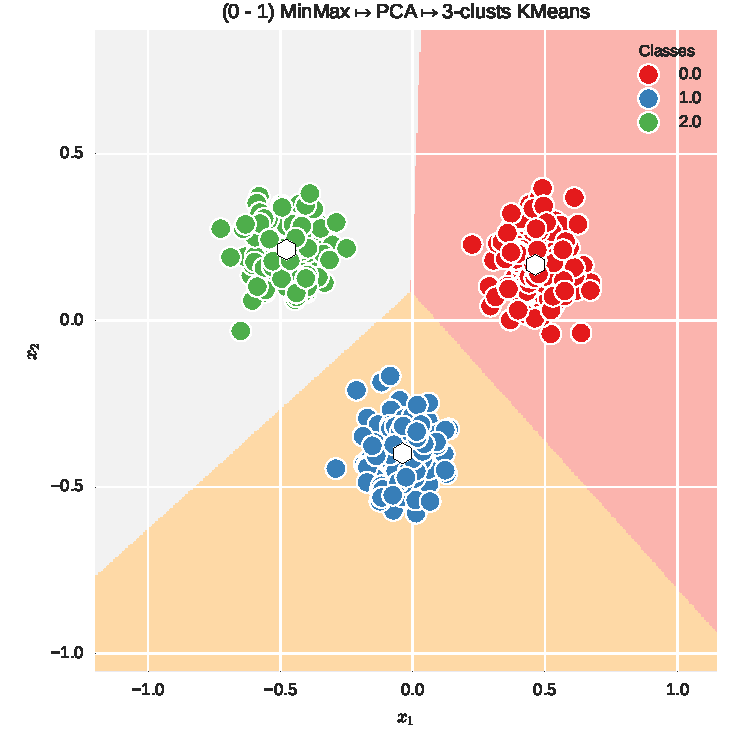
\includegraphics{_static/KMeans.png}
\end{figure}


\section{API}
\label{index:api}\label{index:id1}

\subsection{Pipeline utilities}
\label{index:module-adenine.core.define_pipeline}\label{index:pipeline-utilities}\index{adenine.core.define\_pipeline (module)}\index{DummyNone (class in adenine.core.define\_pipeline)}

\begin{fulllineitems}
\phantomsection\label{index:adenine.core.define_pipeline.DummyNone}\pysigline{\strong{class }\code{adenine.core.define\_pipeline.}\bfcode{DummyNone}}
Dummy class that does nothing.

It is a sklearn `transforms', it implements both a fit and a transform method and it just returns the data in input. It has been created only for consistency with sklearn.

\end{fulllineitems}

\index{parse\_preproc() (in module adenine.core.define\_pipeline)}

\begin{fulllineitems}
\phantomsection\label{index:adenine.core.define_pipeline.parse_preproc}\pysiglinewithargsret{\code{adenine.core.define\_pipeline.}\bfcode{parse\_preproc}}{\emph{key}, \emph{content}}{}
Parse the options of the preprocessing step.

This function parses the preprocessing step coded as dictionary in the ade\_config file.
\begin{quote}\begin{description}
\item[{Parameters}] \leavevmode
\textbf{key} : \{`None', `Recenter', `Standardize', `Normalize', `MinMax'\}
\begin{quote}

The type of selected preprocessing step.
\end{quote}

\textbf{content} : list, len
\begin{quote}

A list containing the On/Off flag and a nested list of extra parameters (e.g. {[}min,max{]} for Min-Max scaling).
\end{quote}

\item[{Returns}] \leavevmode
\textbf{pptpl} : tuple
\begin{quote}

A tuple made like that (`PreprocName', preprocObj), where preprocObj is an sklearn `transforms' (i.e. it has bot a .fit and .transform method).
\end{quote}

\end{description}\end{quote}

\end{fulllineitems}

\index{parse\_dimred() (in module adenine.core.define\_pipeline)}

\begin{fulllineitems}
\phantomsection\label{index:adenine.core.define_pipeline.parse_dimred}\pysiglinewithargsret{\code{adenine.core.define\_pipeline.}\bfcode{parse\_dimred}}{\emph{key}, \emph{content}}{}
Parse the options of the dimensionality reduction step.

This function does the same as parse\_preproc but works on the dimensionality reduction \& manifold learning options.
\begin{quote}\begin{description}
\item[{Parameters}] \leavevmode
\textbf{key} : \{`None', `PCA', `KernelPCA', `Isomap', `LLE', `SE', `MDS', `tSNE'\}
\begin{quote}

The selected dimensionality reduction algorithm.
\end{quote}

\textbf{content} : list, len
\begin{quote}

A list containing the On/Off flag and a nested list of extra parameters (e.g. {[}'rbf,'poly'{]} for KernelPCA).
\end{quote}

\item[{Returns}] \leavevmode
\textbf{drtpl} : tuple
\begin{quote}

A tuple made like that (`DimRedName', dimredObj), where dimredObj is an sklearn `transforms' (i.e. it has bot a .fit and .transform method).
\end{quote}

\end{description}\end{quote}

\end{fulllineitems}

\index{parse\_clustering() (in module adenine.core.define\_pipeline)}

\begin{fulllineitems}
\phantomsection\label{index:adenine.core.define_pipeline.parse_clustering}\pysiglinewithargsret{\code{adenine.core.define\_pipeline.}\bfcode{parse\_clustering}}{\emph{key}, \emph{content}}{}
Parse the options of the clustering step.

This function does the same as parse\_preproc but works on the clustering options.
\begin{quote}\begin{description}
\item[{Parameters}] \leavevmode
\textbf{key} : \{`KMeans', `KernelKMeans', `AP', `MS', `Spectral', `Hierarchical'\}
\begin{quote}

The selected dimensionality reduction algorithm.
\end{quote}

\textbf{content} : list, len
\begin{quote}

A list containing the On/Off flag and a nested list of extra parameters (e.g. {[}'rbf,'poly'{]} for KernelKMeans).
\end{quote}

\item[{Returns}] \leavevmode
\textbf{cltpl} : tuple
\begin{quote}

A tuple made like that (`ClusteringName', clustObj), where clustObj implements the .fit method.
\end{quote}

\end{description}\end{quote}

\end{fulllineitems}

\index{parse\_steps() (in module adenine.core.define\_pipeline)}

\begin{fulllineitems}
\phantomsection\label{index:adenine.core.define_pipeline.parse_steps}\pysiglinewithargsret{\code{adenine.core.define\_pipeline.}\bfcode{parse\_steps}}{\emph{steps}}{}
Parse the steps and create the pipelines.

This function parses the steps coded as dictionaries in the ade\_config files and creates a sklearn pipeline objects for each combination of imputing -\textgreater{} preprocessing -\textgreater{} dimensinality reduction -\textgreater{} clustering algorithms.
\begin{description}
\item[{A typical step may be of the following form:}] \leavevmode
stepX = \{`Algorithm': {[}On/Off flag, {[}variant0, ...{]}{]}\}

\end{description}

where On/Off flag = \{True, False\} and variantX = `string'.
\begin{quote}\begin{description}
\item[{Parameters}] \leavevmode
\textbf{steps} : list of dictionaries
\begin{quote}

A list of (usually 4) dictionaries that contains the details of the pipelines to implement.
\end{quote}

\item[{Returns}] \leavevmode
\textbf{pipes} : list of sklearn.pipeline.Pipeline
\begin{quote}

The returned list must contain every possible combination of imputing -\textgreater{} preprocessing -\textgreater{} dimensionality reduction -\textgreater{} clustering algorithms. The maximum number of pipelines that could be generated is 20, even if the number of combinations is higher.
\end{quote}

\end{description}\end{quote}

\end{fulllineitems}

\phantomsection\label{index:module-adenine.core.pipelines}\index{adenine.core.pipelines (module)}\index{create() (in module adenine.core.pipelines)}

\begin{fulllineitems}
\phantomsection\label{index:adenine.core.pipelines.create}\pysiglinewithargsret{\code{adenine.core.pipelines.}\bfcode{create}}{\emph{pdef}}{}
Scikit-learn Pipelines objects creation (deprecated).

This function creates a list of sklearn Pipeline objects starting from the list of list of tuples given in input that could be created using the adenine.core.define\_pipeline module.
\begin{quote}\begin{description}
\item[{Parameters}] \leavevmode
\textbf{pdef} : list of list of tuples
\begin{quote}

This arguments contains the specification needed by sklearn in order to create a working Pipeline object.
\end{quote}

\item[{Returns}] \leavevmode
\textbf{pipes} : list of sklearn.pipeline.Pipeline objects
\begin{quote}

The list of Piplines, each of them can be fitted and trasformed with some data.
\end{quote}

\end{description}\end{quote}

\end{fulllineitems}

\index{which\_level() (in module adenine.core.pipelines)}

\begin{fulllineitems}
\phantomsection\label{index:adenine.core.pipelines.which_level}\pysiglinewithargsret{\code{adenine.core.pipelines.}\bfcode{which\_level}}{\emph{label}}{}
Define the step level according to the input step label.

This function return the level (i.e.: imputing, preproc, dimred, clustring, None) according to the step label provided as input.
\begin{quote}\begin{description}
\item[{Parameters}] \leavevmode
\textbf{label} : string
\begin{quote}

This is the step level as it is reported in the ade\_config file.
\end{quote}

\item[{Returns}] \leavevmode
\textbf{level} : \{imputing, preproc, dimred, clustering, None\}
\begin{quote}

The appropriate level of the input step.
\end{quote}

\end{description}\end{quote}

\end{fulllineitems}

\index{evaluate() (in module adenine.core.pipelines)}

\begin{fulllineitems}
\phantomsection\label{index:adenine.core.pipelines.evaluate}\pysiglinewithargsret{\code{adenine.core.pipelines.}\bfcode{evaluate}}{\emph{level}, \emph{step}, \emph{X}}{}
Transform or predict according to the input level.

This function uses the transform or the predict method on the input sklearn-like step according to its level (i.e. imputing, preproc, dimred, clustering, none).
\begin{quote}\begin{description}
\item[{Parameters}] \leavevmode
\textbf{level} : \{`imputing', `preproc', `dimred', `clustering', `None'\}
\begin{quote}

The step level.
\end{quote}

\textbf{step} : sklearn-like object
\begin{quote}

This might be an Imputer, or a PCA, or a KMeans (and so on...) sklearn-like object.
\end{quote}

\textbf{X} : array of float, shape
\begin{quote}

The input data matrix.
\end{quote}

\item[{Returns}] \leavevmode
\textbf{res} : array of float
\begin{quote}

A matrix projection in case of dimred, a label vector in case of clustering, and so on.
\end{quote}

\end{description}\end{quote}

\end{fulllineitems}

\index{run() (in module adenine.core.pipelines)}

\begin{fulllineitems}
\phantomsection\label{index:adenine.core.pipelines.run}\pysiglinewithargsret{\code{adenine.core.pipelines.}\bfcode{run}}{\emph{pipes=()}, \emph{X=()}, \emph{exp\_tag='def\_tag'}, \emph{root='`}}{}
Fit and transform/predict some pipelines on some data.

This function fits each pipeline in the input list on the provided data. The results are dumped into a pkl file as a dictionary of dictionaries of the form \{`pipeID': \{`stepID' : {[}alg\_name, level, params, data\_out, data\_in, model\_obj, voronoi\_suitable\_object{]}, ...\}, ...\}. The model\_obj is the sklearn model which has been fit on the dataset, the voronoi\_suitable\_object is the very same model but fitted on just the first two dimensions of the dataset. If a pipeline fails for some reasons the content of the stepID key is a list of np.nan.
\begin{quote}\begin{description}
\item[{Parameters}] \leavevmode
\textbf{pipes} : list of list of tuples
\begin{quote}

Each tuple contains a label and a sklearn Pipeline object.
\end{quote}

\textbf{X} : array of float, shape
\begin{quote}

The input data matrix.
\end{quote}

\textbf{exp\_tag} : string
\begin{quote}

An intuitive tag for the current experiment.
\end{quote}

\textbf{root} : string
\begin{quote}

The root folder to save the results.
\end{quote}

\textbf{parallel} : bool
\begin{quote}

Run all the pipelines in parallel on the cores of your machine (if True, it requires pplus).
\end{quote}

\item[{Returns}] \leavevmode
\textbf{outputFolderName} : string
\begin{quote}

The path of the output folder.
\end{quote}

\end{description}\end{quote}

\end{fulllineitems}

\phantomsection\label{index:module-adenine.core.analyze_results}\index{adenine.core.analyze\_results (module)}\index{make\_scatter() (in module adenine.core.analyze\_results)}

\begin{fulllineitems}
\phantomsection\label{index:adenine.core.analyze_results.make_scatter}\pysiglinewithargsret{\code{adenine.core.analyze\_results.}\bfcode{make\_scatter}}{\emph{root=()}, \emph{embedding=()}, \emph{model\_param=()}, \emph{trueLabel=nan}}{}
Generate and save the scatter plot of the dimensionality reduced data set.

This function generates the scatter plot representing the dimensionality reduced data set. The plots will be saved into the root folder in a tree-like structure.
\begin{quote}\begin{description}
\item[{Parameters}] \leavevmode
\textbf{root} : string
\begin{quote}

The root path for the output creation
\end{quote}

\textbf{embedding} : array of float, shape
\begin{quote}

The low space embedding estimated by the dimensinality reduction and manifold learning algorithm.
\end{quote}

\textbf{model\_param} : dictionary
\begin{quote}

The parameters of the dimensionality reduciont and manifold learning algorithm.
\end{quote}

\textbf{trueLabel} : array of float, shape
\begin{quote}

The true label vector; np.nan if missing (useful for plotting reasons).
\end{quote}

\end{description}\end{quote}

\end{fulllineitems}

\index{make\_voronoi() (in module adenine.core.analyze\_results)}

\begin{fulllineitems}
\phantomsection\label{index:adenine.core.analyze_results.make_voronoi}\pysiglinewithargsret{\code{adenine.core.analyze\_results.}\bfcode{make\_voronoi}}{\emph{root=()}, \emph{data\_in=()}, \emph{model\_param=()}, \emph{trueLabel=nan}, \emph{labels=()}, \emph{model=()}}{}
Generate and save the Voronoi tessellation obtained from the clustering algorithm.

This function generates the Voronoi tessellation obtained from the clustering algorithm applied on the data projected on a two-dimensional embedding. The plots will be saved into the appropriate folder of the tree-like structure created into the root folder.
\begin{quote}\begin{description}
\item[{Parameters}] \leavevmode
\textbf{root} : string
\begin{quote}

The root path for the output creation
\end{quote}

\textbf{data\_in} : array of float, shape
\begin{quote}

The low space embedding estimated by the dimensinality reduction and manifold learning algorithm.
\end{quote}

\textbf{model\_param} : dictionary
\begin{quote}

The parameters of the dimensionality reduciont and manifold learning algorithm.
\end{quote}

\textbf{trueLabel} : array of float, shape
\begin{quote}

The true label vector; np.nan if missing (useful for plotting reasons).
\end{quote}

\textbf{labels} : array of int, shape
\begin{quote}

The result of the clustering step.
\end{quote}

\textbf{model} : sklearn or sklearn-like object
\begin{quote}

An instance of the class that evaluates a step. In particular this must be a clustering model provided with the {\color{red}\bfseries{}clusters\_centers\_} attribute (e.g. KMeans).
\end{quote}

\end{description}\end{quote}

\end{fulllineitems}

\index{est\_clst\_perf() (in module adenine.core.analyze\_results)}

\begin{fulllineitems}
\phantomsection\label{index:adenine.core.analyze_results.est_clst_perf}\pysiglinewithargsret{\code{adenine.core.analyze\_results.}\bfcode{est\_clst\_perf}}{\emph{root=()}, \emph{data\_in=()}, \emph{label=()}, \emph{trueLabel=nan}, \emph{model=()}, \emph{metric='euclidean'}}{}
Estimate the clustering performance.

This function estimate the clustering performance by means of several indexes. Then eventually saves the results in a tree-like structure in the root folder.
\begin{quote}\begin{description}
\item[{Parameters}] \leavevmode
\textbf{root} : string
\begin{quote}

The root path for the output creation
\end{quote}

\textbf{data\_in} : array of float, shape
\begin{quote}

The low space embedding estimated by the dimensinality reduction and manifold learning algorithm.
\end{quote}

\textbf{label} : array of float, shape
\begin{quote}

The label assignment performed by the clusterin algorithm.
\end{quote}

\textbf{trueLabel} : array of float, shape
\begin{quote}

The true label vector; np.nan if missing.
\end{quote}

\textbf{model} : sklearn or sklearn-like object
\begin{quote}

An instance of the class that evaluates a step. In particular this must be a clustering model provided with the {\color{red}\bfseries{}clusters\_centers\_} attribute (e.g. KMeans).
\end{quote}

\end{description}\end{quote}

\end{fulllineitems}

\index{get\_step\_attributes() (in module adenine.core.analyze\_results)}

\begin{fulllineitems}
\phantomsection\label{index:adenine.core.analyze_results.get_step_attributes}\pysiglinewithargsret{\code{adenine.core.analyze\_results.}\bfcode{get\_step\_attributes}}{\emph{step=()}, \emph{pos=()}}{}
Get the attributes of the input step.

This function returns the attributes (i.e. level, name, outcome) of the input step. This comes handy when dealing with steps with more than one parameter (e.g. KernelPCA `poly' or `rbf').
\begin{quote}\begin{description}
\item[{Parameters}] \leavevmode
\textbf{step} : list
\begin{quote}

A step coded by ade\_run.py as {[}name, level, results, parameters{]}
\end{quote}

\textbf{pos} : int
\begin{quote}

The position of the step inside the pipeline.
\end{quote}

\item[{Returns}] \leavevmode
\textbf{name} : string
\begin{quote}

A unique name for the step (e.g. KernelPCA\_rbf).
\end{quote}

\textbf{level} : \{imputing, preproc, dimred, clustering\}
\begin{quote}

The step level.
\end{quote}

\textbf{data\_out} : array of float, shape
\begin{quote}

Where n\_out is n\_dimensions for dimensionality reduction step, or 1 for clustering.
\end{quote}

\textbf{data\_in} : array of float, shape
\begin{quote}

Where n\_in is n\_dimensions for preprocessing/imputing/dimensionality reduction step, or n\_dim for clustering (because the data have already been dimensionality reduced).
\end{quote}

\textbf{param} : dictionary
\begin{quote}

The parameters of the sklearn object implementing the algorithm.
\end{quote}

\textbf{mdl\_obj} : sklearn or sklearn-like object
\begin{quote}

This is an instance of the class that evaluates a step.
\end{quote}

\end{description}\end{quote}

\end{fulllineitems}

\index{make\_tree() (in module adenine.core.analyze\_results)}

\begin{fulllineitems}
\phantomsection\label{index:adenine.core.analyze_results.make_tree}\pysiglinewithargsret{\code{adenine.core.analyze\_results.}\bfcode{make\_tree}}{\emph{root=()}, \emph{data\_in=()}, \emph{model\_param=()}, \emph{trueLabel=nan}, \emph{labels=()}, \emph{model=()}}{}
Generate and save the tree structure obtained from the clustering algorithm.

This function generates the tree obtained from the clustering algorithm applied on the data. The plots will be saved into the appropriate folder of the tree-like structure created into the root folder.
\begin{quote}\begin{description}
\item[{Parameters}] \leavevmode
\textbf{root} : string
\begin{quote}

The root path for the output creation
\end{quote}

\textbf{data\_in} : array of float, shape
\begin{quote}

The low space embedding estimated by the dimensinality reduction and manifold learning algorithm.
\end{quote}

\textbf{model\_param} : dictionary
\begin{quote}

The parameters of the dimensionality reduciont and manifold learning algorithm.
\end{quote}

\textbf{trueLabel} : array of float, shape
\begin{quote}

The true label vector; np.nan if missing (useful for plotting reasons).
\end{quote}

\textbf{labels} : array of int, shape
\begin{quote}

The result of the clustering step.
\end{quote}

\textbf{model} : sklearn or sklearn-like object
\begin{quote}

An instance of the class that evaluates a step. In particular this must be a clustering model provided with the {\color{red}\bfseries{}clusters\_centers\_} attribute (e.g. KMeans).
\end{quote}

\end{description}\end{quote}

\end{fulllineitems}

\index{make\_dendrogram() (in module adenine.core.analyze\_results)}

\begin{fulllineitems}
\phantomsection\label{index:adenine.core.analyze_results.make_dendrogram}\pysiglinewithargsret{\code{adenine.core.analyze\_results.}\bfcode{make\_dendrogram}}{\emph{root=()}, \emph{data\_in=()}, \emph{model\_param=()}, \emph{trueLabel=nan}, \emph{labels=()}, \emph{model=()}}{}
Generate and save the dendrogram obtained from the clustering algorithm.

This function generates the dendrogram obtained from the clustering algorithm applied on the data. The plots will be saved into the appropriate folder of the tree-like structure created into the root folder.
\begin{quote}\begin{description}
\item[{Parameters}] \leavevmode
\textbf{root} : string
\begin{quote}

The root path for the output creation
\end{quote}

\textbf{data\_in} : array of float, shape
\begin{quote}

The low space embedding estimated by the dimensinality reduction and manifold learning algorithm.
\end{quote}

\textbf{model\_param} : dictionary
\begin{quote}

The parameters of the dimensionality reduciont and manifold learning algorithm.
\end{quote}

\textbf{trueLabel} : array of float, shape
\begin{quote}

The true label vector; np.nan if missing (useful for plotting reasons).
\end{quote}

\textbf{labels} : array of int, shape
\begin{quote}

The result of the clustering step.
\end{quote}

\textbf{model} : sklearn or sklearn-like object
\begin{quote}

An instance of the class that evaluates a step. In particular this must be a clustering model provided with the {\color{red}\bfseries{}clusters\_centers\_} attribute (e.g. KMeans).
\end{quote}

\end{description}\end{quote}

\end{fulllineitems}

\index{make\_scatterplot() (in module adenine.core.analyze\_results)}

\begin{fulllineitems}
\phantomsection\label{index:adenine.core.analyze_results.make_scatterplot}\pysiglinewithargsret{\code{adenine.core.analyze\_results.}\bfcode{make\_scatterplot}}{\emph{root=()}, \emph{data\_in=()}, \emph{model\_param=()}, \emph{trueLabel=nan}, \emph{labels=()}, \emph{model=()}, \emph{n\_dimensions=2}}{}
Generate and save the scatter plot obtained from the clustering algorithm.

This function generates the scatter plot obtained from the clustering algorithm applied on the data projected on a two-dimensional embedding. The color of the points in the plot is consistent with the label estimated by the algorithm. The plots will be saved into the appropriate folder of the tree-like structure created into the root folder.
\begin{quote}\begin{description}
\item[{Parameters}] \leavevmode
\textbf{root} : string
\begin{quote}

The root path for the output creation
\end{quote}

\textbf{data\_in} : array of float, shape
\begin{quote}

The low space embedding estimated by the dimensinality reduction and manifold learning algorithm.
\end{quote}

\textbf{model\_param} : dictionary
\begin{quote}

The parameters of the dimensionality reduciont and manifold learning algorithm.
\end{quote}

\textbf{trueLabel} : array of float, shape
\begin{quote}

The true label vector; np.nan if missing (useful for plotting reasons).
\end{quote}

\textbf{labels} : array of int, shape
\begin{quote}

The result of the clustering step.
\end{quote}

\textbf{model} : sklearn or sklearn-like object
\begin{quote}

An instance of the class that evaluates a step. In particular this must be a clustering model provided with the {\color{red}\bfseries{}clusters\_centers\_} attribute (e.g. KMeans).
\end{quote}

\end{description}\end{quote}

\end{fulllineitems}

\index{start() (in module adenine.core.analyze\_results)}

\begin{fulllineitems}
\phantomsection\label{index:adenine.core.analyze_results.start}\pysiglinewithargsret{\code{adenine.core.analyze\_results.}\bfcode{start}}{\emph{inputDict=()}, \emph{rootFolder=()}, \emph{y=nan}, \emph{feat\_names=()}, \emph{class\_names=()}}{}
Analyze the results of ade\_run.

This function analyze the dictionary generated by ade\_run, generates the plots, and saves them in a tree-like folder structure in rootFolder.
\begin{quote}\begin{description}
\item[{Parameters}] \leavevmode
\textbf{inputDict} : dictionary
\begin{quote}

The dictionary created by ade\_run.py on some data.
\end{quote}

\textbf{rootFolder} : string
\begin{quote}

The root path for the output creation
\end{quote}

\textbf{y} : array of float, shape
\begin{quote}

The label vector; np.nan if missing.
\end{quote}

\textbf{feature\_names} : array of integers (or strings), shape
\begin{quote}

The feature names; a range of numbers if missing.
\end{quote}

\textbf{class\_names} : array of integers (or strings), shape
\begin{quote}

The class names; a range of numbers if missing.
\end{quote}

\end{description}\end{quote}

\end{fulllineitems}



\subsection{Input Data}
\label{index:input-data}\label{index:module-adenine.utils.data_source}\index{adenine.utils.data\_source (module)}\index{MixGauss() (in module adenine.utils.data\_source)}

\begin{fulllineitems}
\phantomsection\label{index:adenine.utils.data_source.MixGauss}\pysiglinewithargsret{\code{adenine.utils.data\_source.}\bfcode{MixGauss}}{\emph{mu=()}, \emph{std=()}, \emph{n\_sample=()}}{}
Create a Gaussian dataset.

Generates a dataset with n\_sample * n\_class examples and n\_dim dimensions. Mu, the mean vector, is n\_class x n\_dim.
\begin{quote}\begin{description}
\item[{Parameters}] \leavevmode
\textbf{mu} : array of float, shape
\begin{quote}

The mean of each class.
\end{quote}

\textbf{std} :  array of float, shape
\begin{quote}

The standard deviation of each Gaussian distribution.
\end{quote}

\textbf{n\_sample} : int
\begin{quote}

Number of point per class.
\end{quote}

\end{description}\end{quote}

\end{fulllineitems}

\index{load\_custom() (in module adenine.utils.data\_source)}

\begin{fulllineitems}
\phantomsection\label{index:adenine.utils.data_source.load_custom}\pysiglinewithargsret{\code{adenine.utils.data\_source.}\bfcode{load\_custom}}{\emph{fileName\_X}, \emph{fileName\_y}}{}
Load a custom dataset.

This function loads the data matrix and the label vector returning a unique sklearn-like object dataSetObj.
\begin{quote}\begin{description}
\item[{Parameters}] \leavevmode
\textbf{fileName\_X} : string
\begin{quote}

The data matrix file name.
\end{quote}

\textbf{fileName\_y} : string
\begin{quote}

The label vector file name.
\end{quote}

\item[{Returns}] \leavevmode
\textbf{data} : sklearn.datasets.base.Bunch
\begin{quote}

An instance of the sklearn.datasets.base.Bunch class, the meaningful attributes are .data, the data matrix, and .target, the label vector
\end{quote}

\end{description}\end{quote}

\end{fulllineitems}

\index{load() (in module adenine.utils.data\_source)}

\begin{fulllineitems}
\phantomsection\label{index:adenine.utils.data_source.load}\pysiglinewithargsret{\code{adenine.utils.data\_source.}\bfcode{load}}{\emph{opt='custom'}, \emph{fileName\_X=None}, \emph{fileName\_y=None}}{}
Load a specified dataset.

This function can be used either to load one of the standard scikit-learn datasets or a different dataset saved as X.npy Y.npy in the working directory.
\begin{quote}\begin{description}
\item[{Parameters}] \leavevmode
\textbf{opt} : \{`iris', `digits', `diabetes', `boston', `blobs','custom'\}, default: `custom'

\textbf{fileName\_X} : string, default
\begin{quote}

The data matrix file name.
\end{quote}

\textbf{fileName\_y} : string, default
\begin{quote}

The label vector file name.
\end{quote}

\item[{Returns}] \leavevmode
\textbf{X} : array of float, shape
\begin{quote}

The input data matrix.
\end{quote}

\textbf{y} : array of float, shape
\begin{quote}

The label vector; np.nan if missing.
\end{quote}

\textbf{feature\_names} : array of integers (or strings), shape
\begin{quote}

The feature names; a range of number if missing.
\end{quote}

\end{description}\end{quote}

\end{fulllineitems}



\subsection{Extra tools}
\label{index:extra-tools}\label{index:module-adenine.utils.extra}\index{adenine.utils.extra (module)}\index{modified\_cartesian() (in module adenine.utils.extra)}

\begin{fulllineitems}
\phantomsection\label{index:adenine.utils.extra.modified_cartesian}\pysiglinewithargsret{\code{adenine.utils.extra.}\bfcode{modified\_cartesian}}{\emph{*args}}{}
Modified Cartesian product.

This function takes two (ore more) lists and returns their Cartesian product, if one of the two list is empty this function returns the non-empty one.
\begin{quote}\begin{description}
\item[{Parameters}] \leavevmode
\textbf{*args} : lists, length
\begin{quote}

The group of input lists.
\end{quote}

\item[{Returns}] \leavevmode
\textbf{cp} : list
\begin{quote}

The Cartesian Product of the two (or more) nonempty input lists.
\end{quote}

\end{description}\end{quote}

\end{fulllineitems}

\index{make\_time\_flag() (in module adenine.utils.extra)}

\begin{fulllineitems}
\phantomsection\label{index:adenine.utils.extra.make_time_flag}\pysiglinewithargsret{\code{adenine.utils.extra.}\bfcode{make\_time\_flag}}{}{}
Generate a time flag.

This function simply generates a time flag using the current time.
\begin{quote}\begin{description}
\item[{Returns}] \leavevmode
\textbf{timeFlag} : string
\begin{quote}

A unique time flag.
\end{quote}

\end{description}\end{quote}

\end{fulllineitems}

\index{sec\_to\_time() (in module adenine.utils.extra)}

\begin{fulllineitems}
\phantomsection\label{index:adenine.utils.extra.sec_to_time}\pysiglinewithargsret{\code{adenine.utils.extra.}\bfcode{sec\_to\_time}}{\emph{seconds}}{}
Transform seconds into formatted time string

\end{fulllineitems}



\renewcommand{\indexname}{Python Module Index}
\begin{theindex}
\def\bigletter#1{{\Large\sffamily#1}\nopagebreak\vspace{1mm}}
\bigletter{a}
\item {\texttt{adenine.core.analyze\_results}}, \pageref{index:module-adenine.core.analyze_results}
\item {\texttt{adenine.core.define\_pipeline}}, \pageref{index:module-adenine.core.define_pipeline}
\item {\texttt{adenine.core.pipelines}}, \pageref{index:module-adenine.core.pipelines}
\item {\texttt{adenine.utils.data\_source}}, \pageref{index:module-adenine.utils.data_source}
\item {\texttt{adenine.utils.extra}}, \pageref{index:module-adenine.utils.extra}
\end{theindex}
\renewcommand{\indexname}{Python Module Index}
\begin{theindex}
\def\bigletter#1{{\Large\sffamily#1}\nopagebreak\vspace{1mm}}
\bigletter{a}
\item {\texttt{adenine.core.analyze\_results}}, \pageref{index:module-adenine.core.analyze_results}
\item {\texttt{adenine.core.define\_pipeline}}, \pageref{index:module-adenine.core.define_pipeline}
\item {\texttt{adenine.core.pipelines}}, \pageref{index:module-adenine.core.pipelines}
\item {\texttt{adenine.utils.data\_source}}, \pageref{index:module-adenine.utils.data_source}
\item {\texttt{adenine.utils.extra}}, \pageref{index:module-adenine.utils.extra}
\end{theindex}

\renewcommand{\indexname}{Index}
\printindex
\end{document}
